\documentclass{beamer}
\usepackage{isolatin1}
\usepackage{latexsym}

\usepackage{listings}
\lstset{language=XML,showspaces=false,showtabs=false}

\usepackage[german]{babel}

\usetheme{Berlin}
\mode<presentation>

\title{Integration von RSS mit verteiltem Publish/Subscribe}
\author{Friedemann Zintel}

\begin{document}
\bibliographystyle{ieeetr}

\begin{frame}

  \titlepage

\end{frame}

\section*{Outline}
\begin{frame}

  \tableofcontents

\end{frame}

\section{Einleitung}

\begin{frame}

  \begin{itemize}
    \item Verteilung von Informationen �ber das Internet gewinnt immer mehr an Bedeutung.
    \item Verteilungskonzept: Publish/Subscribe (Pub/Sub)
    \item RSS: Pub/Sub-System, jedoch nicht im herk�mmlichen Sinne
    \item RSS: von viele Anbietern unterst�tzt (beliebt: BLogs)
  \end{itemize}

\end{frame}

\section{�berblick}

\subsection{Publish/Subscribe}
\begin{frame}
  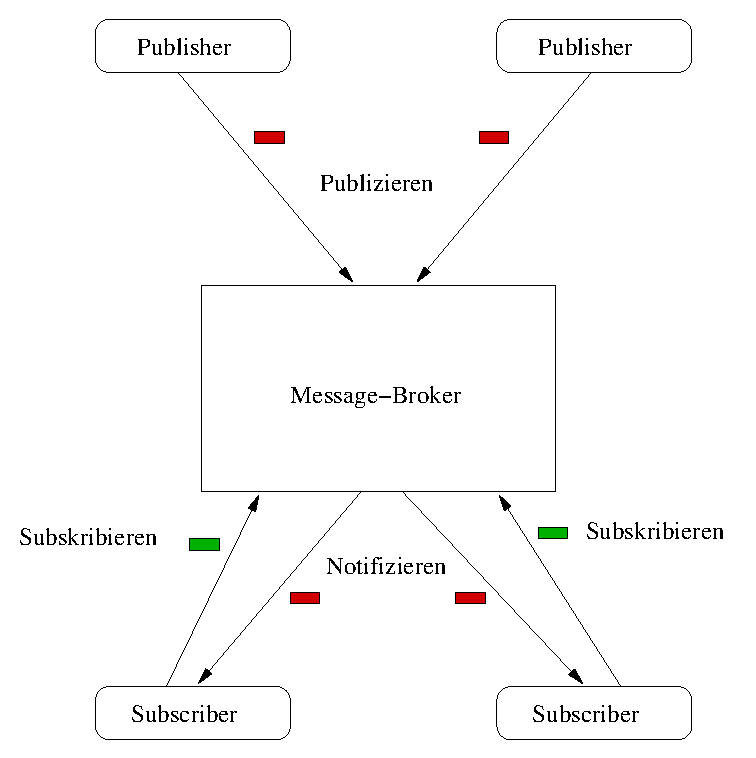
\includegraphics[bb=-50 0 200 350,scale=0.6]{PubSub}
\end{frame}

\subsection{RSS}
\begin{frame}

  \frametitle{RSS: Really Simple Syndication}
  \begin{itemize}
    \item RSS-Feed dient u.a. zur Kurzbeschreibung von Web-News
    \item XML-basiert
    \item Erreichbar durch Link auf Anbieterseite
  \end{itemize}
  \nocite{LiuVenSirer:2005:MeasureRSSPubSub}

\end{frame}

\begin{frame}[fragile,allowframebreaks]
  \frametitle{Beispiel: RSS-Feed}
  \tiny
  \begin{lstlisting}
<?xml version="1.0" encoding="iso-8859-1"?>
<!DOCTYPE rss PUBLIC "-//Netscape Communications//DTD RSS 0.91//EN"
  "http://my.netscape.com/publish/formats/rss-0.91.dtd"> 

<rss version="0.91">

<channel>

 <title>SPIEGEL ONLINE</title>
 <link>http://www.spiegel.de</link>
 <description>Schneller wissen, was wichtig ist</description>
 <language>de</language>

 <image>
  <title>SPIEGEL ONLINE</title>
  <url>http://www.spiegel.de/static/sys/logo_120x61.gif</url>
  <link>http://www.spiegel.de</link>
 </image>
  \end{lstlisting}
  \begin{lstlisting}
 <item>
  <title>Bagdad Sniper:  Der Mann, der Juba &#252;berlebte</title>
  <link>http://www.spiegel.de/panorama/0,1518,394137,00.html</link>
 </item>

 <item>
  <title>Infineon:  Vorstand streitet &#252;ber Speichersparte</title>
  <link>http://www.spiegel.de/wirtschaft/0,1518,394143,00.html</link>
 </item>

 <item>
  <title>Biathlon:  Glagow l&#228;uft Olympiasiegerin davon</title>
  <link>http://www.spiegel.de/sport/wintersport/0,1518,394138,00.html</link>
 </item>

 </channel>
 </rss>
  \end{lstlisting}
  Quelle: www.heise.de
\end{frame}

\section{Motivation}
\begin{frame}

  \frametitle{Anwendersicht: Was man gerne h�tte ...}
  \begin{itemize}
    \item Automatische Benachrichtigung �ber Feed-Updates
    \item Aktualit�t der Feeds
    \item Definition von Filtern auf h�herer Ebene: zur \dots
      \begin{list}{}{}
        \item \dots individuellen Vorselektion der News
	\item \dots anbieter�bergreifenden Zusammenstellung neuer Feeds
      \end{list}
  \end{itemize}

\end{frame}

\begin{frame}

  \frametitle{Stand der Dinge}
  \begin{itemize}
    \item RSS: Kein Pub/Sub im herk�mmlichen Sinne $\rightarrow$ Client/Server
    \item Feeds m�ssen von Anwendersoftware erfragt werden (Polling)
    \item Vordefinierte Channel $\rightarrow$ thematische Zuordnung auf Publisherseite
    \item Definition von Filtern nur auf Anwenderseite m�glich
  \end{itemize}

  \pause
  Probleme:
  \begin{itemize}
    \item Polling:
      \begin{list}{$\longrightarrow$}{}
        \item Gro�er Datenverkehr im Netz
	\item Hohe serverseitige Last
      \end{list}
    \item Filterdefinition nur beim Anwender:
      \begin{list}{$\longrightarrow$}{}
        \item alle Feeds m�ssen heruntergeladen werden
      \end{list}
  \end{itemize}
  \nocite{Hicks:2004:RSSBandwith}
  
\end{frame}

\begin{frame}

  \frametitle{Ziel}
  \begin{itemize}
    \item Entlastung der RSS-Server
    \item Reduzierung des Datenverkehrs aufgrund von Polling
    \item Erh�hung des Aktualit�tsgrades der Feeds auf Nutzerseite
    \item Erm�glichung der subscriber-seitigen Definition von Filtern
  \end{itemize}

\end{frame}

\section{Umsetzung}
\begin{frame}
  \frametitle{Integration von RSS in verteiltes Pub/Sub-System}
  \begin{itemize}
    \item RSS-Server k�nnte als Publisher fungieren
    \item Broker sorgen f�r eine Verteilung der Feeds an Nutzer (Subscriber)
  \end{itemize}

  \pause
  Problem:\\
  Neue Software muss sowohl auf Server-Seite als auch auf Anwenderseite installiert werden.
%    \item Verteilung der RSS-Feeds mittels herk�mmlichem Pub/Sub $\Longrightarrow$ Notifikation der Subscriber
\end{frame}

\begin{frame}
  \frametitle{L�sung:}
\begin{itemize}
  \item Rolle der RSS-Server ver�ndert sich nicht
  \item Nutzer holen Feed in der Rolle des Publisher und speisen ihn in das Broker-Netz
  \item Broker verteilen Feeds an Nutzer bzw. Subscriber
\end{itemize}
\end{frame}

\begin{frame}
  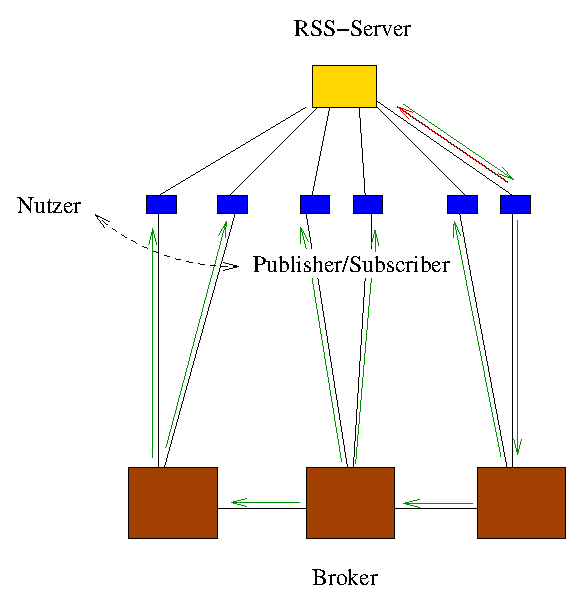
\includegraphics[bb=-100 0 200 250,scale=0.6]{RSSPubSub}
\end{frame}

\begin{frame}
  \frametitle{Ansatz: Ein Publisher}
  \begin{itemize}
    \item Ein Publisher w�rde ausreichen um Feed herunterzuladen
    \item Alle weiteren Nutzer  bzw. Subscriber w�rden den Feed �bers Netzwerk erhalten
  \end{itemize}

  \pause
  Vorteil:\\
  Wenige Anfragen an den RSS-Server
\vspace{0.5cm}
  
  \pause
  Problem:\\
  Aktualit�t der Feeds!\\
  $\longrightarrow$ lange �bertragungszeiten in Abh�ngigkeit von Netzstruktur
\end{frame}

\begin{frame}
  \frametitle{Aktualit�t vs. Server-Belastung}
  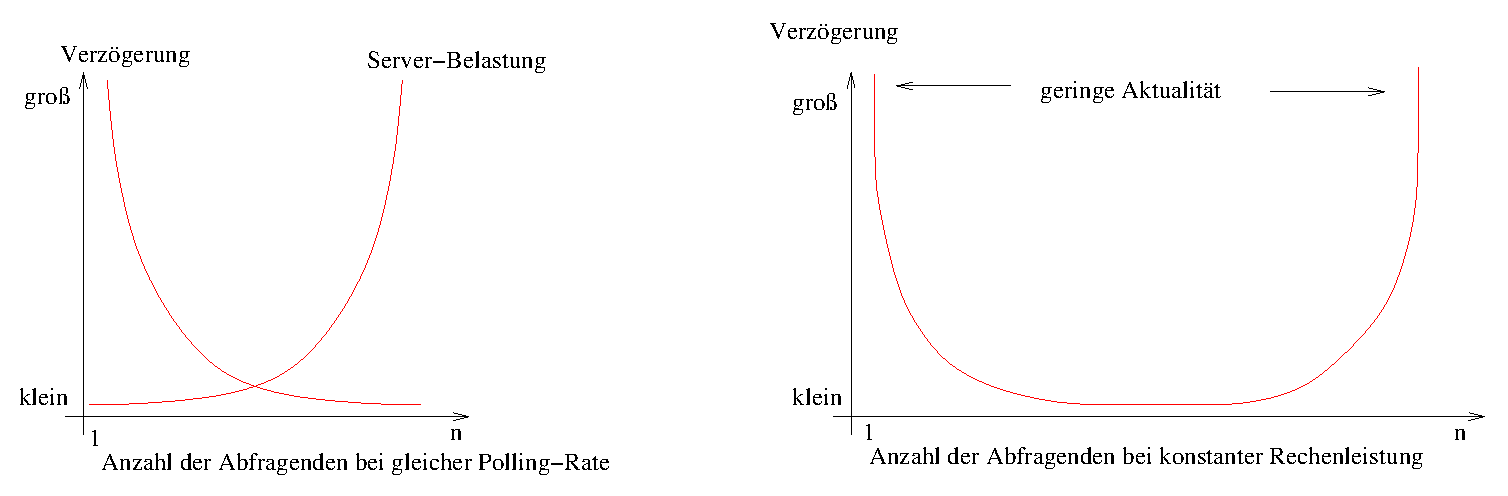
\includegraphics[bb=20 0 200 250,scale=0.5]{Verzoegerung}
\end{frame}

\begin{frame}
  \frametitle{Ansatz: Mehrere Publisher}
  \begin{itemize}
    \item Mehrere Publisher laden Feed herunter
    \item $\rightarrow$ Mindestens so viele, dass gewisse Aktualit�t d. F.'s erreicht wird
    \item $\rightarrow$ H�chstens so viele, dass Server nicht �berlastet wird
  \end{itemize}
\vspace{0.5cm}

$\longrightarrow$ Optimum muss bestimmt werden

\end{frame}

\begin{frame}
  \frametitle{Frage:}
  Wie k�nnen sich die Publisher dar�ber abstimmen, wer als n�chstes den aktuellen Feed abholt?
\end{frame}

\begin{frame}
  \frametitle{Herausforderungen}
Entwicklung von Algorithmen zur \dots
  \begin{itemize}
    \item \dots Koordination der Publisher
    \item \dots Ermittlung der RSS-Server-Auslastung
    \item \dots Bestimmung des Update-Intervalls eines Feeds
    \item \dots Bestimmung der Nachrichtenlaufzeiten (eventuell)
  \end{itemize}
\end{frame}

\section{Literatur}
\begin{frame}[allowframebreaks]
  \bibliography{../bibdatabase}
\end{frame}

\end{document}
